\chapter{Gefaltete neuronale Netze}
\label{kap:CNN}

Feed-Forward-Netze gelten als leistungsstarke maschinelle Lernmethoden, da sie so trainiert werden können, um beliebige komplexe Funktionen abhängig von einer vektorwertigen Eingabe zu approximieren. Ist die Dimension der Eingabeschicht jedoch zu groß, treten bei klassischen FFN Probleme hinsichtlich der Paramteranzahl auf. Die Problemstellung \ref{prob:class_image} dieser Arbeit besteht in der Klassifikation digitalisierter Bilder. Wird ein FFN mit $100$ Ausgabeneuronen genutzt und jeder Pixel eines Bildes mit den Abmessungen $1000 \times 1000$ als Merkmal genutzt, so ergeben sich bereits $10^8+100$ freie Parameter. Stehen nur relativ wenige Traingsdaten zur Verfügung, ist die Struktur des FFN zu komplex und dies kann zur Überanpassung führen\cite{caruana2000overfitting,bilbao2017overfitting}. Die Parameteranzahl muss also deutlich reduziert werden. Konzepte wie \textit{Parameter Sharing} und spärliche Konnektivität, engl. \textit{sparse connectivity} erlauben diese Reduktion, vgl. Goodfellow\cite{Goodfellow-et-al-2016} und werden in den folgenden Abschnitten erläutert.

Ein weiterer Nachteil des FFN ergibt sich dadurch, dass Korrelationen von benachbarten Eingabeneuronen, z.B. Bilsegmente wie Kanten oder Ecken, nicht miteinbezogen werden. Es muss also eine Modell entwickelt werden, welches diese lokalen Muster extrahiert und sie miteinander verknüpft. Das Modell sollte zudem äquivariant gegenüber Translationen sein. 

%Schließlich sind beim FFN die Eingabe- und Ausgabedimension fixiert. Eine flexible Wahl diser Hyperparameter ist bei Problemen der Computergrafik oft erwünscht. 

In diesem Kapitel wird erläutert, wie gefaltete neuronale Netze die erwähnten Nachteile von FFN umgehen. CNN sind in der Lage, lokale Muster zu erkennen, sind äquivariant gegenüber Translationen und realisieren Konzepte wie Parameter Sharing, um die Anzahl der freien Parameter drastisch zu reduzieren. So gelingt es, besonders bei Aufgaben der Computergrafik\cite{DBLP:conf/nips/KrizhevskySH12, DBLP:journals/pieee/LeCunBBH98,DBLP:conf/cvpr/CiresanMS12} die Generalisierungsrate gegenüber klassichen FFN zu erhöhen. 

Gefaltete neuronale Netze unterscheiden sich von FFN bei der Berechnung der Übertragungsfunktion. Dazu wird die gefaltete Übertragungsfunktion definiert, welche das Konzept der diskreten Faltung nutzt. Im folgenden Abschnitt \ref{abs:conv_theorie}wird zunächst die Faltung als mathematische Operation eingeführt und deren Zusammenhang zur Fourier-Transformation\cite{werner2011funktionalanalysis} erläutert. Anschließend wird im Abschnitt \ref{abs:conv_def} das CNN-Modell definiert und schließlich im Abschnitt \ref{abs:CNN_train} der Backpropagationsalgorithmus \ref{alg:online_backprop} auf CNN verallgemeinert.

%bei CNNs zu verstehen ist und wie diese Operation bei diesen neuronalen Netzen motiviert wird. In diesem Zusammenhang werden Begriffe wie Merkmalskarten (engl. \textit{feature maps}) und Filter (engl. \textit{kernels}) eingeführt. Des Weiteren wird die Arithmetik der Faltungsoperation für zweidimensionale Eingaben, repräsentiert durch Matrizen, erklärt und das Verfahren \textit{padding} beziehungsweise das Nutzen von \textit{strides} erläutert. Das gesamte Kapitel wird mit konkreten Beispielen begleitet, um die verschiedenen Effekte der Faltungsoperation zu beleuchten.

\section{Die Faltungsoperation}
\label{abs:conv_theorie}
In der Analysis ist die Faltung ein mathematischer Operator und liefert für zwei Funktionen $f$ und $g$ die Funktion $ f \ast g$, wobei mit dem Sternchen die Faltungsoperation gemeint ist.

\begin{defi}[Faltung]\label{allg_faltung}
    Für zwei Funktionen $f,g: \Rnv \rightarrow \mathbb{C}$ ist die Faltung als
    \begin{equation*}
        (f \ast g) (x) := \int_{\Rnv} f(\tau) g(x-\tau) \mathrm{d} \tau
    \end{equation*}
    definiert, wobei gefordert wird, dass das Integral für fast alle $x$ wohldefiniert ist. Für $f,g \in L^1(\RR^n)$ ist dies der Fall.
   \end{defi}

Für die Faltung gelten einige Rechenregeln.

\begin{lem}
    \label{lem:convrules}
    Seien $f,g,h \in L^1(\RR^n)$ und $a \in \mathbb{C}$. Dann gelten
    \begin{align*}
         (i) \; \; &f \ast g = g \ast f \; \; &( \text{Kommutativität}) \\
         (ii) \; \; &f \ast (g \ast h) = (f \ast g) \ast h  \; \;& (\text{Assoziativität}) \\
         (iii) \; \; &f \ast (g+h) = (f+g) \ast h \; \; &(\text{Distributivität}) \\ 
         (iv) \; \; &a(f \ast g) = (af) \ast g = f \ast (ag) \; \; &(\text{Assoziativität mit skalarer Multiplikation}) 
    \end{align*}
\end{lem}

\begin{proof}
    Eine Beweis dieser Rechenregeln kann in Werner\cite{werner2011funktionalanalysis} nachgelsen werden.
\end{proof}

%Bei klassischen neuronalen Netzen, siehe Kapitel \ref{classicNN} werden Eingabedaten durch eine Verkettung von affinen Transformationen verarbeitet. Typischerweise wird die Eingabe als Vektor dargestellt und  mit einer Matrix multipliziert, gegebenenfalls mit einem Biasvektor manipuliert und schließlich so die Ausgabe generiert. Bilder-, Audio- oder Videoaufnahmen besitzen jedoch mehrere Merkmale in unterschiedlichen Achsen. Oft sind solche Eingabedaten im Bereich des Machine-Learnings als mehrdimensionale Arrays abgelegt, welche eine oder mehrere Achsen repräsentieren, wobei die Ordnung dieser eine Rolle spielt. Bei digitalisierten Bildern sind das bespielsweise die Höhe und Breite des Bildes, bei Audioaufnahmen gibt es nur eine Achse, und zwar die Zeitachse. Hinzu kommen Kanalachsen als weitere Verfeinerung der Daten, zum Beispiel besitzen RGB-Farbbilder drei Kanäle der Farben rot, grün und blau. 

%Diese speziellen Eigenschaften können bei affinen Transformationen nicht berücksichtigt werden. Alle Merkmale sowie Achsen werden gewissermaßen gleich behandelt und die wesentliche topologische Struktur kann so nicht zum Vorteil ausgenutzt werden. Hier soll nun die sogenannte diskrete Faltung Abhilfe schaffen.
In der digitalen Signal- und Bildverarbeitung werden meist diskrete Funktionen analysiert und daher die diskrete Faltung genutzt, bei der statt der Intgration eine Summation auftaucht. Die Regeln aus Lemma \ref{lem:convrules} gelten analog.

\begin{defi}[Diskrete Faltung]\label{disk_faltung}
    Für zwei Funktionen $f,g: D \rightarrow \mathbb{C}$ mit einem diskreten Definitionsbereich $D \subseteq \mathbb{Z}^n$ ist die diskrete Faltung als
    \begin{equation*}
        (f \ast g) (n) := \sum_{k \in D} f(k) g(x-k)
    \end{equation*}
    definiert. Hier wird über dem gesamten Definitionsbereich $D$ summiert. Ist $D$ beschränkt, werden $f$ beziehungsweise $g$ durch Nullen fortgesetzt.  
\end{defi}

Ist für $f,g: D \rightarrow \mathbb{C}$ der Definitionsbereich $D$ endlich, so können die Funktionen als zeitdiskrete Signale $f=(f_0, \ldots, f_{n-1})^T \in \mathbb{C}^{n}$ und $g=(g_0, \ldots, g_{n-1})^T \in \mathbb{C}^{n}$ aufgefasst werden. %Durch das Fortsetzen mit Nullen besitzen die Vektoren $f$ und $g$ die gleiche Länge. 
In diesem Fall kann die Faltung als Matrix-Vektor-Produkt mit einer zyklischen Matrix ausgedrückt werden. 

\begin{defi}[Zyklische Matrix, vgl. Gray\cite{gray2006toeplitz}]
    Eine quadratische Matrix heißt zyklisch im Vektor $a=(a_0, \ldots, a_{n-1})^T \in \RR^n$, wenn sie die Gesatlt
    \begin{equation*}
        \mathrm{zyk}(a):=
        \begin{pmatrix}
            a_0 & a_{n-1} &a_{n-2} &\ldots &a_1 \\ 
            a_1 & a_0 &a_{n-1} & \ldots &a_2 \\
            a_2 & a_1 &a_0 & \ldots &a_3 \\
             &\ddots &\ddots &\ddots & \\
            a_{n-1} &a_{n-2} &a_{n-3} &\ldots &a_0
        \end{pmatrix}
    \end{equation*}
    besitzt.
\end{defi}    
    
\begin{bem}
Für ein zeitdiskrete Signal $f=(f_0, \ldots, f_{n-1})^T \in \mathbb{C}^{n}$ sei $F=\mathrm{zyk}(f)$ die zyklische Matrix im Vektor $f$. Sei weiter $g=(g_0, \ldots, g_{n-1})^T \in \mathbb{C}^{n}$. Dann lässt sich mit
    \begin{equation*}
        (F g)_k=\sum_{j=0}^{n-1}  f_{k-j} g_j,  \; \; k=0, \ldots, n-1
    \end{equation*}
    die diskrete Faltung von $f$ und $g$ darstellen. Dabei werden Indizies außerhalb von $0, \ldots, n-1$ zyklisch durch Modulo-Rechnung ($\mathrm{mod} \; n)$ in den gültigen Indexbereich abgebildet.
\end{bem}

In Hinblick auf die Klassifikation von digitalisierten Bildern, dargestellt als Matrizen, wird die Matrixfaltung mit sogenannten quadratischen Kernen $K \in \RR^{k \times k}$ mit ungeradem $k \in \mathbb{N}$ definiert.
 
%Um die Notation einfach zu halten, sei ein Kern $K$ ebenfalls eine $h \times b$ - Matrix, indem $K$ mit Nullen aufgefüllt wird.

%\begin{defi}[Zweidimensionale Faltung]
    %Sei $X \in \RR^{h \times b}$ und $K \in \RR^{k \times k}$. Das Ergebnis der zweidimensionalen Faltung ist die Matrix $Y= X \ast K \in \RR^{h \times b}$ mit

%    \begin{equation}
%        \label{eq:2dmatrixconv}
%        Y_{i,j}= \sum_{p \in [k]} \sum_{q \in [k]} X_{p,q} K_{p-i+3,q-j+3}.
%    \end{equation}
%    Dabei besitzt $Y$ die selben Abmessungen wie $X$. 
%\end{defi}

\begin{defi}[Matrixfaltung, vgl. \cite{gruening}] \label{def:matrix_faltung}
    Für gegebene Matrizen $X \in \RR^{h \times b}$ und $K \in \RR^{k \times k}$ sei $u=\lfloor k/2  \rfloor$.
    %\begin{equation*}
    %   h_l=\begin{cases}
    %       \lfloor k_h/2  \rfloor &, k_h \, \text{ungerade} \\
    %       k_h/2-1 &, \text{sonst}
    %    \end{cases}, \; \; 
    %    w_l=\begin{cases}
    %        \lfloor k_w/2 \rfloor &, k_w \, \text{ungerade} \\
    %        k_w/2 -1 &, \text{sonst}    
    %    \end{cases}.
    %\end{equation*} 
    Die zweidimensionale Faltung  $Y=X \ast K \in \RR^{h \times w}$ ist als 
    \begin{equation}
        \label{eq:matrix_faltung}
        (Y)_{i,j}:=\sum_{l=-u}^{u} \sum_{m=-u}^{u} X_{i+l,j+m} K_{l+u+1, m+u+1}\; \; \forall i \in [h], j \in [b]
    \end{equation} mit $X_{i,j}=0$ für $i \notin [h]$ und $j \notin [b]$ definiert. In der Literatur wird dieses Auffüllen mit Nullen am Rand von $X$ mit \textit{zero padding} bezeichnet. In dieser Definition besitzt das Ergebnis $Y$ der Faltung die gleichen Abmessungen wie $X$.
\end{defi}

Bei gefalteten neuronalen Netzen wird oft eine Reduktion der Dimensionen angestrebt. Dafür werden natürliche Zahlen als Schrittweiten, engl. \textit{strides}, genutzt.
\begin{bem}\label{bem_strides}
    Für Schrittweiten $s_h, s_b \in \mathbb{N}$ ergibt sich die reduzierte zweidimensionale Faltung $Y=X \ast K$ zu
    \begin{equation*}
        (Y)_{i,j}:=\sum_{l=-u}^{u} \sum_{m=-u}^{u} X_{i \cdot s_h +l,j \cdot s_b +m} K_{l+u+1, m+u+1}\; \; \forall i \in [\lceil h/s_h \rceil], j \in [\lceil b/s_b \rceil].
    \end{equation*}
    Für $s_h=s_b=1$ ergibt sich die Standardvariante wie in \ref{eq:matrix_faltung}.
    \end{bem}

\section{CNN Architektur}

Beim maschinellen Lernen sind Eingabedaten oft als mehrdimensionale Arrays abgelegt, welche eine oder mehrere Achsen repräsentieren, wobei die Ordnung dieser eine Rolle spielt. Bei digitalisierten Bildern sind das bespielsweise die Höhe und Breite des Bildes, welche als Raumachsen bezeichnet werden. Hinzu kommen Kanalachsen, zum Beispiel besitzen Grauwert-Bilder einen Farbkanal, während RGB-Farbbilder drei Kanäle der Farben rot, grün und blau besitzen. Dementsprechend werden Grauwert-Bilder wie in Definition \ref{def:image} nun als dreidimensionale Arrays $X \in [0,1]^{h \times b \times 1}$ dargestellt. Dies erlaubt die Definition der gefalteten Übertragungsfunktion, wie in Gruening\cite{gruening}

\begin{defi}[Gefaltete Übertragungsfunktion]
    \label{eq:convlogit}
    Sei ein vierdimensionales Array $K \in \RR^{z_{out} \times z_{in} \times k \times k}$ und ein Biasvektor $b \in \RR^{z_{out}}$ gegeben. Die Funktion 
    \begin{equation*}
        \Psi_{conv}^{K,b}: \RR^{\cdot \times \cdot \times z_{in}} \rightarrow \RR^{\cdot \times \cdot\times z_{out}}
    \end{equation*}
    mit
    \begin{equation*}
        \Psi_{conv}^{K,b}(X)_{:,:,q}:= \sum_{p=1}^{z_{in}} \alpha_p\left(K_{q,p,:,:} \ast X_{:,:,p} \right) +b_q \; \forall q \in [z_{out}]
    \end{equation*}
    wird gefaltete Übertragungsfunktion bezeichnet. Mit $\ast$ ist die Matrixfaltung wie in Definition \ref{def:matrix_faltung} gemeint und mit $\cdot$ werden beliebige Raumachsen bezeichnet. Die Skalare $\alpha_p$ sind lernbare Parameter. In dieser Arbeit gelte $\alpha_p=1$ für alle $p \in [z_{in}]$.
\end{defi}


\begin{bem}
    Ist $\psi: \RR \rightarrow \RR$ eine Aktivierungsfunktion wie in Definition \ref{def_act_f}, so wird für $X \in \RR^{\cdot \times \cdot \times z}$ mit 
    \[\psi(X)_{i,j,:}:=\left(\psi(X_{i,j,1}), \ldots, \psi(X_{i,j,z})\right)^T \in \RR^z \; \; \forall i \in [{}_1 X], j \in [{}_2 X] 
    \]
    der Vektor bezeichnet, welcher sich durch die elementweise Auswertung der Aktivierungsfunktion $\psi$ ergibt.
\end{bem}

Ähnlich der Definition \ref{def:NNlayer} wird nun eine Faltungsschicht als Verknüpfung von gefalteter Übertragungsfunktion und Aktivierungsfunktion definiert.

\begin{defi}[Faltungsschicht]
    \label{def:convlayer}
    Ist $\Psi_{conv}^{K,b}$ eine gefaltete Übertragungsfunktion und $\psi$ eine Aktivierungsfunktion, so wird das Paar $(\Psi_{conv}^{K,b}, \psi)$ als Faltungsschicht $\mathcal{S}_{conv}$ bezeichnet. Für eine sogenannte Eingabekarte $X \in \RR^{\cdot \times \cdot \times z_{in}}$ ist die Ausgabe $Y \in \RR^{\cdot \times \cdot \times z_{out}}$ der Schicht $\mathcal{S}_{conv}$ durch
    \[Y=\psi \circ \Psi_{conv}^{K,b}(X)= \psi\left(\Psi_{conv}^{K,b}(X)\right)
        \] 
        gegeben. Die Matrizen $Y_{:,:,p}$ werden für $1 \leq p \leq z_{out}$ Merkmalskarten genannt. Weiter bezeichne $\Psi_{conv}^{K^{},b^{},\psi_{}}$ die Faltungsschicht $\mathcal{S}_{conv}$ mit $\Psi_{conv}^{K^{},b^{},\psi_{}}(X):= \psi_{} \left(\Psi_{conv}^{K^{},b^{}}(X)\right)$.
\end{defi}

Bei CNN werden sogenannte \textit{Pooling}-Schichten verwendet, um die Dimensionen der Raumachsen neben dem zero padding weiter zu verkleinern und das Modell robuster gegenüber Überanpassung zu machen. Dazu werden Pooling-Funktionen eingesetzt, welche unabhängig voneinander auf Merkmalskarten operieren und so die Rechenkomplexität des Modells reduzieren. Es ist sinnvoll, symmetrische Pooling-Funktionen $T$ zu wählen, für die die Bedingung
\begin{equation*}
    \forall \pi \in S_n \; \forall x \in \RR^n: T(x_1, \ldots, x_n)=T(x_{\pi(1)}, \ldots, x_{\pi(n)})
\end{equation*}
gilt. Mögliche Pooling-Funktionen sind 
\begin{alignat*}{2}
    \text{Maximum}: \; \;&T(x_1, \ldots x_n) &&= \max\{x_1, \ldots x_n\},\\
    \text{Mittelwert}: \; \;&T(x_1, \ldots, x_n) &&= \frac{1}{n} \sum_{i=1}^n x_i. 
 \end{alignat*}
Heutzutage wird oft die von Weng et. al.\cite{weng1992cresceptron} eingeführte Max-Pooling-Schicht benutzt.
Für den späteren Trainingsprozess ist es nützlich, die Ableitung der verwendeten Pooling-Funktionen, sofern sie existiert, zur Verfügung zu haben. Für den Mittelwert $T$ gilt $\nabla T=\frac{1}{n} \textbf{1}$. Ist $T$ die Maximum-Funktion so ergibt sich

\begin{equation*}
    \frac{\partial T}{\partial x_i}= \begin{cases}
        1 , \; \text{falls}  \; \forall j \neq i: \; x_i >x_j \\
        0 , \; \text{falls}  \; \exists j \neq i: \; x_i <x_j
    \end{cases}
\end{equation*}
mit der Konvention, dass für $x_1=x_2= \ldots=x_n$ die Ableitung auf $\frac{1}{2}
$ gesetzt wird. Pooling-Schichten werden wieder durch Schrittweiten parametrisiert.

\begin{defi}[Pooling-Schicht, vgl. Grüning \cite{gruening}]
    Seien $p_h, p_b \in \mathbb{N}$ und $T$ eine Pooling-Funktion. Die Funktion 
    \begin{equation*}
        \Psi_{pool,T}^{p_h,p_b}: \RR^{\cdot \times \cdot \times z} \rightarrow \RR^{\cdot \times \cdot\times z}
    \end{equation*}
    mit
    \begin{equation*}
        \Psi_{pool,T}^{p_h,p_b}(X)_{i,j,l}:= \mathop{T}_{\begin{subarray}{l}(i-1) \cdot p_h < i' \leq \min\{i \cdot p_h, {}_1 X\} \\ 
        (j-1) \cdot p_w < j' \leq \min\{j \cdot p_w, {}_2 X\}\end{subarray}} (X_{i',j',l})  
    \end{equation*}
    für alle  $i \in [\lceil {}_1 X/p_h \rceil], j \in [\lceil {}_2 X/p_w \rceil]$ und $l \in [z]$ wird Pooling-Schicht genannt. Die Schrittweiten $p_h, p_b \in \mathbb{N}$ werden subsampling-Faktoren genannt.
\end{defi}

Pooling-Schichten verdichten also Information von Eingabedaten, welche sich lokal in Fenstern der Größe $p_h \times p_b$ befinden und reduzieren so die Raumdimension. In dieser Arbeit wird das Maximum-Pooling oder Mittelwert-Pooling benutzt. Für andere Pooling-Funktion sei auf Yu et. al.\cite{yu2014mixed} verwiesen.
Die Idee bei CNN besteht nun darin, Faltungsschichten mit Pooling-Schichten zu kombinieren und schließlich ein FFN wie in Definition \ref{def:MLP} anzuknüpfen.
Dazu wird für allgemeine mehrdimensionale Arrays die Flatten-Schicht definiert.

\begin{defi}
    \label{def:flatten}
    Sei $X \in \RR^{n_1 \times n_2 \times n_3}$. Dann wird die Funktion $T_f:\RR^{n_1 \times n_2 \times n_3} \rightarrow \RR^{n_1 \cdot n_2 \cdot n_3}$ mit 
    \begin{equation*}
        T_f(X)_{(i-1) \cdot (n_2 \cdot n_3)+(j-1) \cdot n_3+k}:= X_{i,j,k}, \; \; \forall i \in [n_1],\; j \in [n_2],\; k \in [n_3]
    \end{equation*}
    Flatten-Funktion genannt. Die multidimensionale Eingabe wird also in einen Vektor umgewandelt.
\end{defi}

Dies erlaubt die Definition des CNN-Modells als Kombination aus Faltungsschichten, Pooling-Schichten und Neuronenschichten des MLP aus Kapitel \ref{kap:NN}. 
\begin{defi}(Gefaltetes Neuronales Netz)
    Seien $h, w, z_{in}, z_{out}, l ,c \in \mathbb{N}$ und Schichten $\Psi^{W^{(1)},b^{(1)},\psi_{1}}, \ldots, \Psi^{W^{(l)},b^{(l)},\psi_{l}}$ sowie Faltungsschichten $\Psi_{conv}^{K^{(1)},b^{(1)},\psi_{1}}, \ldots, \Psi_{conv}^{K^{(l)},b^{(l)},\psi_{l}}$ gegeben. Die Vorwärtsrechnung eines CNN lässt sich als Komposition
    \begin{equation}
        \label{eq:CNN_for}
        y=\Psi^{W^{(l)},b^{(l)},\psi_{l}} \circ \ldots \circ \Psi^{W^{(1)},b^{(1)},\psi_{1}} \circ T_f \circ \Psi_{conv}^{K^{(c)},b^{(c)},\psi_{c}} \circ \ldots \circ \Psi_{conv}^{K^{(1)},b^{(1)},\psi_{l}}(X)
    \end{equation} 
    darstellen. Dabei seien wieder die Dimensionen der Parameter passend gewählt, sodass die Komposition wohldefiniert ist. In (\ref{eq:CNN_for}) können zwischen den Faltungsschichten Pooling-Schichten $\Psi_{pool,T}^{p_h,p_b}(X)$ geschaltet werden.
\end{defi}
Auch CNN bestehen aus Hyper- und Modellparametern.

\begin{defi}[Hyper- und Modellparameter von CNN]
    Die Eingabe- und Ausgabedimensionen $h, b, z_{in}, z_{out}$, die Anzahl $c$ der Faltunsschichten, dei Anzahl $l$ der Neuronenschichten, die Dimensionen der Kerne, die Schrittweiten bei der Faltung bzw. dem Pooling sowie die verwendeten Aktivierungs- und Poolingfunktionen sind Hyperparameter des CNN.
    Die Kerne, Gewichtsmatrizen und Biasvektoren mit den entsprechend passenden Abmessungen stellen die Modellparameter $\mathcal{W}:=\{(W^{(i)},b^{(i)}): \; i=1, \ldots, l\}$ und $\mathcal{W}_{conv}:=\{(K^{(i)}, b^{(i)}): \; i=1, \ldots, c\}$ des CNN dar. 
\end{defi}
Die Hyperparameter werden wieder anwendungsspezifisch für das jeweilige Problem gewählt und die Modellparameter während des Trainingsprozesses angepasst. 


\section{Backpropagation bei CNN}
\label{abs:CNN_train}
Der Backpropagationsalgorithmus \ref{alg:online_backprop} soll nun für das CNN-Modell verallgemeinert werden. 
Als Fehlerfunktion wird wieder die mittlere quadratische Abweichung (\ref{eq:MSE})
genutzt. 
Die Abstiegsrichtungen für die Schichten des FFN wurden bereits im vorherigen Kapitel \ref{kap:NN} hergeleitet. Es müssen nun Gradienten innerhalb der Faltungsschichten beziehungsweise Pooling-Schichten berechnet werden. Die Einträge der Eingabe- und Merkmalskarten, in Zukunft einfach Karten genannt, können als Neuronenaktivierungen interpretiert werden. Weiter werden zur Vereinfachung die trainierbaren Gewichte der Kerne in Zukunft mit $w_{i,j}^{(l)}$ bezeichnet. Gemeint ist also das Gewicht zwischen Neuron $i$ auf Schicht $l-1$ und Neuron $j$ der Schicht $l$ bezeichnet. Weiter sei $y_{i}^{(l-1)}$ die Aktivierung des Neurons $i$ der Schicht $l-1$ und $\delta_j^{(l)}$ sei der lokale Fehler des Neurons $j$ der Schicht $l$. Die Funktion $\psi$ repräsentiert eine Aktivierungsfunktion, Pooling-Funktion oder Flatten-Funktion, je nachdem auf welcher Schicht sie benutzt wird.

Die Gradienten werden wieder komponentenweise berechnet.
Angenommen, $l$ ist eine Faltungsschicht. Die Aktivierung einer Merkmalskarte $j$ an der Stelle $(x,y)$ lässt sich mit der Matrixfaltung, siehe \ref{def:matrix_faltung}, \ref{eq:convlogit}, als
\begin{equation}
    y_j^{(l)}(x,y) =\psi \left(\sum_{i \in [z_{in}]} \sum_{(u,v) \in F} y_i^{(l)}(x+u,y+u)\,  w_{j,i}^{(l)}(u,v) +b_j^{(l)}\right)
\end{equation}   
schreiben. Es ist zu beachten, dass $(x,y)$ ein Pixel der Karte $j$ meint. Dabei ist $F=\{(u,v): \; 0\leq u,v <k\}$ und $k$ die Dimension der Kerns.
Das Gewicht des Kerns von der Karte $i$ zur Karte $j$ an der Stelle $(u,v)$ ist mit $w_{j,i}(u,v)$ bezeichnet. Der Gradient ergibt sich als Summe über das Produkt der jeweilgen Positionen $(x,y)$ der Merkmalskarte $j$ und dem lokalen Fehler $\delta^{(l)}_j$, also
\begin{equation}
    \label{eq:CNN_K_grad}
    \Delta w_{j,i}^{(l)}(u,v)= -\lambda \, \sum_{(x,y)} \left( y_i^{(l-1)}(x+u,y+v) \delta_j^{(l)}(x,y)\right)
\end{equation}
Der Zusammenhang in Gleichung (\ref{eq:CNN_K_grad}) ist in Abbildung \ref{abb:error_conv} grafisch dargestellt. Analog ergibt sich für den Schwellwert

\begin{equation*}
    \Delta b_j^{(l)}= -\lambda \, \sum_{(x,y)} \delta_j^{(l)}(x,y).
\end{equation*}
Die Berechnung des lokalen Fehlers $\delta_{j}^{(l)}$ der Schicht $l$ ist abhängig von der Schicht $l+1$.
$V_k=\sum_{j} w_{k,j}^l z_j +b^l_k$ 

\section{Anwendung bei der Ziffernerkennung}
In diesem Abschnitt wird ein CNN zur Klassifikation von Grauwert-Bildern aus einem konkreten Datensatz vorgestellt. Der MNIST-Datensatz\cite{DBLP:journals/pieee/LeCunBBH98} bietet $60.000$ Trainingsbilder handgeschriebener Ziffern und $10.000$ Testbilder, welche jeweils durch menschliches Wissen annotiert sind. Dieser Datensatz gilt als typischer Benchmark zur Klassifikation von Ziffern und wird im weiteren Verlauf dieser Arbeit genutzt. Jedes einzelne Bild besteht aus $28 \times 28$ Pixeln, welche jeweils einen Grauwert zwischen 0 und 1 annehmen, vgl. Abbildung \ref{mnistpic}. Ein Bild wird als $X \in [0,1]^{28 \times 28 \times 1}$ und ein Trainingspaare als $(X,c)$ mit $c \in \{0, \ldots, 9\}$ bezeichnet. 

\begin{figure}[h]
    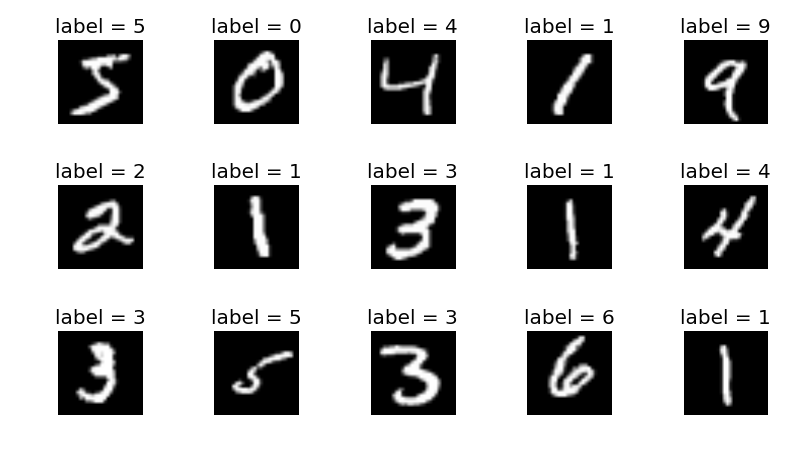
\includegraphics[width=0.8\textwidth]{pics/chapters/CCN/mnist.png}
    \centering
    \caption{Beispielbilder, vgl. \cite{DBLP:journals/pieee/LeCunBBH98} aus der öffentlichen MNIST-Datenbank. Zu sehen sind handgeschriebene Ziffern und zugehörige Annotationen.}
    \label{mnistpic}
\end{figure}

Es wird ein CNN mit zwei Faltungsschichten $C^1$ und $C^2$ mit der logistischen Aktivierungsfunktion $\psi$ genutzt. Die Ausgabe der Schicht $C^1$ umfasst sechs Merkmalskarten und die Ausgabe der Schicht $C^2$ zwölf Merkmalskarten. Zur Faltung werden quadratische $5 \times 5$ -Kerne verwendet. Außerdem werden zwei Pooling-Schichten $P^1$ und $P^2$mit den Schrittweiten $p_h=p_b=2$ und der Mittelwert-Funktion genutzt. Anschließend wird ein FFN mit 10 Ausgabeneuronen angekoppelt, sodass dessen Aktivierung zur Klassifikation der Eingabe genutzt werden kann. Die Architektur, ähnlich dem Le-Net-5-Modell\cite{DBLP:journals/pieee/LeCunBBH98}, ist in Abbildung \ref{abb_CNN_arch} dargestellt. Dabei sind

\begin{itemize}
    \item $X$ ein Grauwert-Bild der Größe $h=b=28$,
    \item $K^1 \in \RR^{6 \times 1 \times 5 \times 5}$ der Kern der Schicht $C^1$,
    \item $b^1 \in \RR^6$ der Biasvektor der Schicht $C^1$,
    \item $K^2 \in \RR^{12 \times 6 \times 5 \times 5}$ der Kern der Schicht $C^2$,
    \item $b^2 \in \RR^{12}$ der Biasvektor der Schicht $C^2$,
    \item $W \in \RR^{192 \times 10}$ die Gewichtsmatrix der Neuronenschicht,
    \item $b \in \RR^{10}$ der Biasvektor der Neuronenschicht,
    \item $y \in \RR^{10}$ die Ausgabe des CNN. 
\end{itemize}

Im Folgenden wird der Online-Backpropagationsalgorithmus \ref{alg:online_backprop_CNN} verwendet, um das CNN zu trainieren. Dieser besteht zunächst aus der Initialisierung und der Vorwärtsrechnung. Zur Übersicht wird im Folgenden eine komponentenweise Schreibweise genutzt.

\section*{Vorwärtsrechnung}

Alle Biasvektoren werden als Nullvektor initialisiert. Zur Initialisierung der Gewichte wird die Xavier-Initialisierung \ref{def:xavier} genutzt, also

\begin{alignat*}{2}
    K^{1}_{p,1}(u,v) &\sim  \mathcal{N} \left(0, \frac{2}{5 \cdot 5 \cdot (1+6)}\right), \; \; &&1 \leq p \leq 6,\\
    K^{2}_{q,p}(u,v) &\sim  \mathcal{N} \left(0, \frac{2}{5 \cdot 5 \cdot (6+12)}\right),\; \; &&1 \leq q \leq 12, 1 \leq p \leq 6,\\
    W(i,j) &\sim \mathcal{N} \left(0, \frac{2}{192+10}\right).
\end{alignat*}
Die Parameteranzahl ist damit 
\begin{equation*}
    \underbrace{(5 \cdot 5 +1) \cdot 6}_{\text{Gewichte in $C^1$}}+\underbrace{(5 \cdot 5 \cdot 6+1) \cdot 12}_{\text{Gewichte in $C^2$}}+\underbrace{(192+1 \cdot 10)}_{\text{Gewichte im FFN}}=3898.
\end{equation*}
 Sei $X \in \RR^{28 \times \times 1}$ das Eingabebild und $\psi$ die logistische Funktion. In der Schicht $C^1$ werden sechs Merkmalskarten 

\begin{align}
    \label{eq:C1_forw}
    \begin{split}
    C_p^1 &= \psi(X \ast K_{p,1}^1+b_p^1 \mathbf{1}) \\
    C_p^1(i,j)&=\psi \left(\sum_{u=0}^4 \sum_{v=0}^4 X(i+u,j+v) \cdot K_{p,1}^1(u,v) +b_p^1\right)
    \end{split}
\end{align}
für $1 \leq p \leq 6$ berechnet. Mit $\mathbf{1} \in \RR^{24 \times 24}$ ist die Matrix gemeint, deren Einträge nur Einsen sind. Die Matrixfaltung $\ast$ wird ohne zero padding genutzt und daher reduziert sich die Raumdimension. Es gilt $C^1_p \in \RR^{24 \times 24 \times 1}$. Anschließend folgen das Mittelwert-Pooling $P^1$ mit
\begin{equation}
    \label{eq:P1_forw}
    P^1_p(i,j) =\frac{1}{4} \sum_{u=0}^1 \sum_{v=0}^1 C_p^1(2i-u, 2j-v), \; i,j \in [12]
\end{equation}
für $1 \leq p \leq 6$ und die zweite Faltungsschicht $C^2$, welche zwölf Merkmalskarten
\begin{align}
    \label{eq:C2_forw}
    \begin{split}
        C_q^2 &= \psi \left( \sum_{p=1}^6 P_p^1 \ast K_{q,p}^2 + \mathbf{1} b_q^2\right) \\
        C_q^2(i,j) &= \psi \left( \sum_{p=1}^6 \sum_{u=0}^4 \sum_{v=0}^4 P^1_p(i+u,j+v) \cdot K_{q,p}(u,v) +b_q^2\right)
    \end{split}
\end{align}
für $1 \leq q \leq 12$ berechnet. Die Matrixfaltung $\ast$ wird wieder ohne zero padding genutzt und daher reduziert sich die Raumdimension.
Es gilt $C_q^2 \in \RR^{8 \times 8 \times 1}$. Es folgt das Mittelwert-Pooling $P^2$ mit
\begin{equation}
    \label{eq:P2_forw}
    P_q^2(i,j)= \frac{1}{4} \sum_{u=0}^1 \sum_{v=0}^1 C_p^1(2i-u, 2j-v), \; i,j \in [4]
\end{equation}
für $1 \leq q \leq 12$. Es gilt $P^2\in \RR^{4 \times 4 \times 12}$. Diese zwölf $4 \times 4$- Matrizen werden durch die Flatten-Funktion $T_f$ aus Definition \ref{def:flatten} in einen Vektor $f \in \RR^{4 \cdot 4 \cdot 12}$ umgewandelt. Dies sei durch
\begin{equation}
    \label{eq:f_forw}
    f=T_f(P^2)
\end{equation}
beschrieben. 
Die Umkehrung wird mit
\begin{equation}
    \label{eq_f_ford_inv}
    P^2=T_f^{-1}(f).
\end{equation}
bezeichnet.
Die Ausgabe des FFN ergibt sich schließlich zu
\begin{equation}
    \label{eq:y_forw}
    y=\psi(W^T f +b).
\end{equation}
und der mittlere quadratische Fehler lautet
\begin{equation}
    \label{eq:E_forw}
    E_{X}=\frac{1}{2} \sum_{k=1}^{10} \left(y(k)-t(k)\right)^2,
\end{equation}
wobei $t=t(X,c)$ der Zielvektor des Datenpaars $(X,c)$ ist.

\section*{Backpropagation}
Zuerst werden die Gradienten bezüglich der Gewichtsmatrix und Biasvektor der Neuronenschicht des FNN berechnet. Es gilt
\begin{align}
    \begin{split}
        \Delta W(j,k) &= -\lambda \, \frac{\partial E}{\partial W(j,k)}\\
                       &= -\lambda \, \frac{\partial L}{\partial y(k)} \cdot \frac{\partial y(k)}{\partial W(j,k)}\\
                       &=-\lambda \, (y(k)-t(k)) \cdot \frac{\partial}{\partial W(j,k)} \psi \left(\sum_{j=1}^{192} W(j,k) f(j)+b(k)\right)\\
                       &=-\lambda \, (y(k)-t(k)) \cdot y(k)(1-y(k)) \cdot f(j).
     \end{split}
\end{align}
Mit $\delta^{\text{FFN}}(k)=(y(k)-t(k)) \cdot y(k)(1-y(k))$ für $1 \leq k \leq 10$ lässt sich $\Delta W$ als dyadisches Produkt  
\begin{align*}
    \Delta W(j,k)&=-\lambda \, \left(\delta^{\text{FFN}}(k) \cdot f(j) \right) \\
    \Rightarrow  \Delta W&=-\lambda \,\left(f \otimes (\delta^{\text{FFN}})^T\right)   
\end{align*}
darstellen. Analog gilt
\begin{equation*}
\Delta b= -\lambda \delta^{\text{FFN}}.
\end{equation*}
Um $ \Delta K_{q,p}$ in $C^2$ zu bestimmen, sind zunächst die lokalen Fehler der darüberliegenden Schicht zu ermitteln. Der lokale Fehler $\delta^f \in \RR^{}$in der Flatten-Schicht lautet
\begin{align*}
    \delta^f(j) &= - \lambda \, \frac{\partial E}{\partial f} \\
                &= - \lambda \, \sum_{k=1}^{10} \frac{\partial E}{\partial y(k)} \cdot \frac{\partial y(k)}{f(j)} \\
                &= - \lambda \, (y(k)-t(k)) \cdot \frac{\partial}{\partial f(j)} \psi \left(\sum_{j=1}^{192} W(k,j) f(j) +b(k)\right) \\
                &=- \lambda \, \sum_{k=1}^{10} (y(k)-t(k)) \cdot y(k)(1-y(k)) \cdot W(k,j) \\
                &=-\lambda \,\sum_{k=1}^{10} \delta^{\text{FFN}}(k) \cdot W(k,j) \\
                \Rightarrow \delta^f &= -\lambda \, W^T \delta^{\text{FFN}}
\end{align*}
In der Pooling-Schicht $P^2$ sind keine Gradienten zu bestimmen, da diese nicht von den Modellparametern abhängt. Mit
\begin{equation}
    \delta^{P^2}=T_f^{-1}(\delta_f) \in \RR^{4 \times 4 \times 12}
\end{equation}
folgt mit $\nabla T=\frac{1}{4} \mathbf{1}$ das Upsampling
\begin{equation}
    \delta^{C^2}(i,j)= \nabla T() \delta_{P^2}\left( \lceil i/2 \rceil, \lceil j/2 \rceil\right)
\end{equation}
%Im Folgenden werden konkrete Beispiele für verschiedene zweidimensionale Faltungen, welche in dieser Arbeit im Fokus stehen, gegeben. Dabei sind die Eingabe $X \in \RR^{h \times w}$ und der Filter $K \in \RR^{k_h \times k_w}$ immer als Matrizen zu verstehen. Das Ergebnis der Faltung $S= X \ast K$ wird als Merkmalskarte bezeichnet. Es sei angemerkt, dass oft $k_h=k_w$ sowie $k_h$ ungerade gewählt wird, z.B. $k_h=3$ oder $k_h=5$. Die Größe der Merkmalskarte wird durch die Parameter
%\begin{itemize}
%    \item $h,w$: Die Höhe und Breite der Eingabe,
%    \item $k_h, k_w$: Die Abmessungen des Filters,
%   \item $s_h, s_w$: Die Wahl der strides, 
%   \item $p_h, p_w$: Die Größe des zero paddings
%\end{itemize}
%beeinflusst. Mit zero padding ist gemeint, dass künstliche Nullen um Randpixel der Eingabe $X$ eingefügt werden, damit die Berechnung mit dem Filter um jene Pixel gelingt. Ein Beispiel für das Verwenden von zero padding wird in Abbildung \ref{abb_simplematrixconv_padding} gezeigt. In Abbildung \ref{abb_simplematrixconv} ist die Berechnung einer einfachen zweidimensionalen Matrixfaltung dargestellt. Ein vorher festgelegter Filter (grau) bewegt sich über die Eingabe (blau) und berechnet jeweils die Einträge der Ausgabe(grün). 

\begin{figure}[h]
    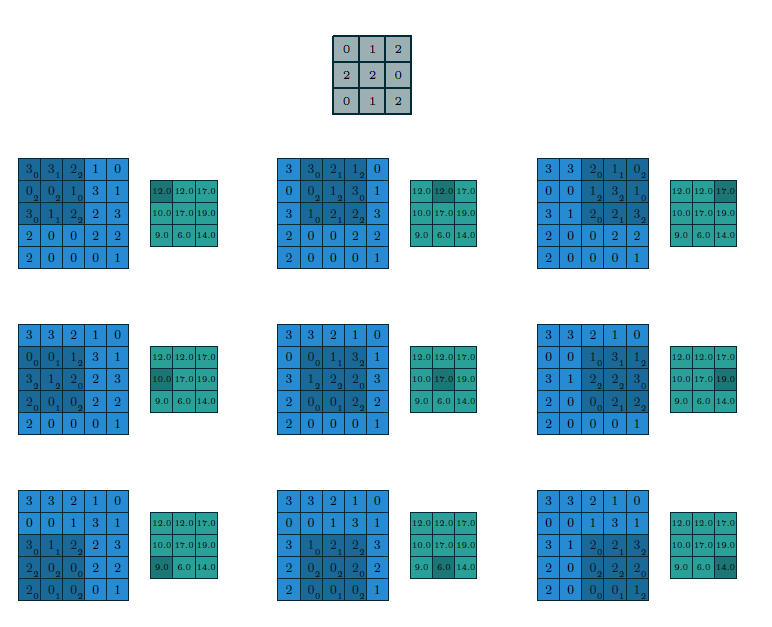
\includegraphics[width=0.8\textwidth]{pics/abb_simpleconv}
    \centering
    \caption{Es wird die Merkmalskarte $S \in \RR^{3 \times 3}$ mit den Parametern ${h,w=5}, k_h=k_w=3, s_h=s_w=1$ und $p_h=p_w=1.$}
    \label{abb_simplematrixconv}
\end{figure}

\begin{figure}[h]
    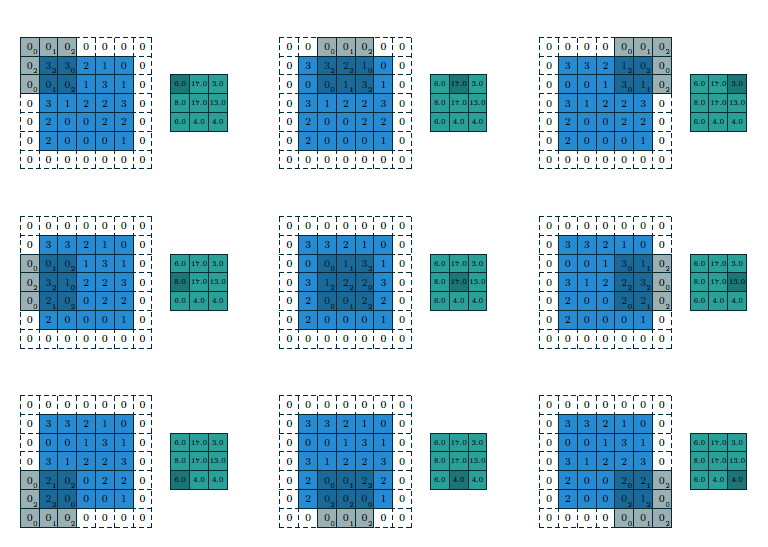
\includegraphics[width=0.8\textwidth]{pics/abb_simplecov_padding}
    \centering
    \caption{Es wird die Merkmalskarte $S \in \RR^{3 \times 3}$ mit den Parametern ${h,w=5}, k_h=k_w=3, s_h=s_w=2$ und $p_h=p_w=1$ berechnet.}
    \label{abb_simplematrixconv_padding}
\end{figure}



\section{Motivation der Faltung}
..
Sie nutzt wichtige Konzepte zur Optimierung von Machine-Learning-Verfahren wie spärliche Konnektivität (engl. \textit{sparse connectivity}), \textit{Parameter Sharing} und \textit{äquivariante Repräsentation}, vgl. \cite{goodfellow}. Spärliche Konnektivität bedeutet, dass Neuronen auf einer Schicht $\mathcal{s}_{l+1}$ nur durch wenige Neuronen der Schicht $\mathcal{S}_l$ beeinflusst wird. Dies ist bei CNNs typisch, da meist die verwendeten Filter viel kleiner als die Eingabe ist. Noch mehr erklären + Abbildung

Mit Parameter Sharing ist die Nutzung von gleichen Parametern für mehrere Funktionen im neuronalen Netz gemeint. In herkömmlichen Feed-Forward-Netzen wird jedes Element der Gewichtsmatrizen für die Berechnung der Aktivierungen der jeweiligen Schichten verwendet. Anschließend werden diese Gewichte dann nicht mehr gebraucht. Im Zusammenhang von CNNs bedeutet Parameter Sharing während der Faltungsoperation, dass nur eine bestimmte Menge von Parametern erlernt werden müssen
Noch mehr erklären + Abbildung

